\chapter{Đường cong elliptic}

Đường cong elliptic (elliptic curve) rất nổi tiếng trong toán học. Đây là
công cụ giúp các nhà toán học giải quyết bài toán lớn \textit{Định lý 
cuối cùng của Fermat}. Trong mật mã học, đường cong elliptic là một
trong những tiêu chuẩn bảo mật về mã hóa và chữ ký điện tử. Chương này 
khảo sát những đặc trưng cơ bản đường cong elliptic và ứng dụng trong
mật mã học.

\section{Mở đầu về đường cong elliptic}

Đường cong elliptic là tập hợp các điểm $(x, y)$ trên mặt phẳng $Oxy$
thỏa mãn phương trình $y^2 = x^3 + ax + b$, với $a, b \in \RR$ và
$4a^3 + 27b^2 \neq 0$.

Ví dụ với phương trình $y^2 = x^3 + 8$, đồ thị được biểu diễn 
ở hình \ref{ecc:1}.

Ví dụ với phương trình $y^2 = x^3 - x$, đồ thị được biểu diễn
ở hình \ref{ecc:2}.

Hoặc đối với phương trình $y^2 = x^3 - 3x + 3$ thì đồ thị được biểu diễn
ở hình \ref{ecc:3}.

Ta thấy rằng, đường cong elliptic đối xứng qua trục hoành.

\begin{figure}[ht]
    \centering
    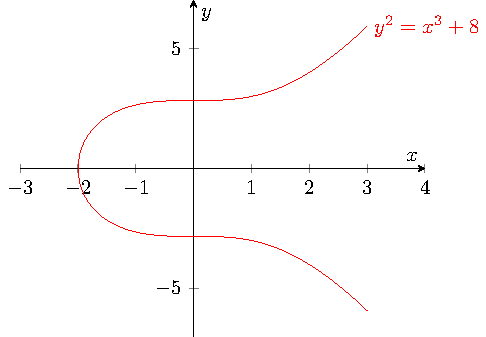
\includegraphics{../pics/ecc/ecc1.pdf}
    \caption{Elliptic $y^2 = x^3 + 8$}
    \label{ecc:1}
\end{figure}

\begin{figure}[ht]
    \centering
    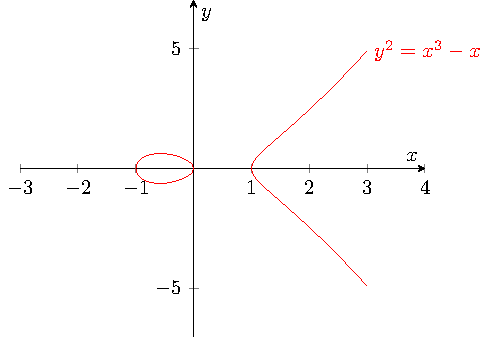
\includegraphics{../pics/ecc/ecc2.pdf}
    \caption{Elliptic $y^2 = x^3 - x$}
    \label{ecc:2}
\end{figure}

\begin{figure}[ht]
    \centering
    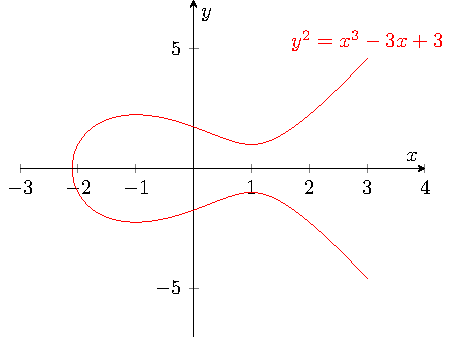
\includegraphics{../pics/ecc/ecc3.pdf}
    \caption{Elliptic $y^2 = x^3 - 3x + 3$}
    \label{ecc:3}
\end{figure}

\section{Phép cộng các điểm trên elliptic}

Phương trình và đồ thị của đường cong elliptic đã được trình bày ở trên.
Tuy nhiên chúng ta quan tâm tới mối liên hệ giữa các điểm trên elliptic, 
cụ thể là phép "cộng" 2 điểm.

Ta thêm một điểm trừu tượng vào tập hợp các điểm trên đường cong
elliptic và gọi là \textbf{điểm vô cực}. Điểm vô cực được ký hiệu là
$\mathcal{O}$.

Khi đó, với điểm $P=(x, y)$ bất kì trên elliptic, điểm đối xứng của
nó qua trục hoàng là $P'=(x,-y)$ và ta định nghĩa $P + P'=\mathcal{O}$.
Tiếp theo ta định nghĩa phép cộng hai điểm.

Giả sử $P=(x_P, y_P)$ và $Q=(x_Q, y_Q)$ là hai điểm trên elliptic.
Ta có hai trường hợp:

\begin{enumerate}
    \item Nếu $P \neq Q$, ta vẽ đường thẳng đi qua $P$ và $Q$. Đường thẳng
    này cắt elliptic tại điểm thứ ba là $S$. Ta lấy $R$ đối xứng với $S$ qua
    trục hoành. Khi đó $R$ cũng nằm trên elliptic và $P + Q = R$;
    \item Nếu $P \equiv Q$, ta vẽ tiếp tuyến với elliptic tại điểm $P$.
    Tiếp tuyến này cắt elliptic tại điểm thứ hai là $S$. Tương tự ta lấy
    $R$ đối xứng với $S$ qua trục hoành. Khi đó $P + Q = 2P = R$.
\end{enumerate}

Khi đó, tập hợp các điểm trên elliptic cùng với điểm vô cực, và phép
cộng hai điểm được định nghĩa như trên tạo thành một nhóm.

Để chứng minh đây là nhóm, ta cần chuyển các khái niệm hình học kia
sang đại số để tính toán và chứng minh.

\subsection*{Phép cộng hai điểm khác nhau}

Đầu tiên ta thiết lập công thức phép cộng giữa hai điểm cho trường 
hợp $P \neq Q$. Giả sử $P = (x_P, y_P)$ và $Q = (x_Q, y_Q)$.

Phương trình đường thẳng đi qua $P$ và $Q$ là

\begin{equation}
    \label{eqecc:1}
    y = \frac{y_Q - y_P}{x_Q - x_P} (x - x_P) + y_P
\end{equation}

Thay $y$ vào phương trình đường cong elliptic ta có

\begin{equation}
    \label{eqecc:2}
    \Big[\frac{y_Q - y_P}{x_Q - x_P} (x - x_P) + y_P\Big]^2 = x^3 + ax + b
\end{equation}

Đặt $k = \dfrac{y_Q - y_P}{x_Q - x_P}$. Khi đó phương trình tương đương
với 
\[(k x - k x_P + y_P)^2 = x^3 + ax + b\]

Khai triển và chuyển vế ta có
\begin{equation}
    x^3 - k^2 x^2 + \ldots = 0
\end{equation}

Ta chỉ cần quan tâm hệ số trước $x^2$. Bởi vì ta biết rằng đường thẳng $PQ$ 
cắt elliptic tại 3 điểm $P$, $Q$, $S$, nên phương trình bậc 3 này có 3 nghiệm 
phân biệt là $x_P$, $x_Q$ và $x_S$ nên theo theo định lý Vieta ta có
\begin{equation*}
    x_P + x_Q + x_S = k^2
\end{equation*}

Như vậy ta có hoành độ điểm $S$
\begin{equation}
    x_S = k^2 - x_P - x_Q
\end{equation}

Thay $x_S$ vào \ref{eqecc:1}, ta có tung độ điểm $S$

\begin{equation}
    y_S = k(x_S - x_P) + y_P
\end{equation}

Mà $R$ đối xứng với $S$ qua trục hoành, như vậy $x_R = x_S$ và $y_R = -y_S$.
Như vậy kết quả của phép cộng là
\begin{align*}
    x_R & = k^2 - x_P - x_Q \\
    y_R & = k(x_P - x_R) - y_P
\end{align*}
với $k = \dfrac{y_Q - y_P}{x_Q - x_P}$.

\subsection*{Phép cộng hai điểm giống nhau}

Trong trường hợp hai điểm giống nhau, ta vẽ tiếp tuyến tiếp xúc với
elliptic đi qua điểm đó. Giả sử ta muốn vẽ tiếp tuyến tại 
điểm $P = (x_P, y_P)$, khi đó từ phương trình elliptic
$y^2 = x^3 + ax + b$ ta vi phân hai vế thu được
\begin{equation}
    2y \,dy = (3x^2 + a) \,dx
\end{equation}

Ta biết rằng hệ số góc của đường tiếp tuyến là đạo hàm hàm số
tại điểm đó, hay nói cách khác là $\,dy/\,dx$. Như vậy hệ số góc
tiếp tuyến tại điểm $P$ là
\begin{equation}
    k = \frac{dy}{dx} = \frac{3 x_P^2 + a}{2y_P}
\end{equation}
và như vậy phương trình đường tiếp tuyến là

\begin{equation}
    y = k(x-x_P) + y_P
\end{equation}

Thực hiện tương tự như bên trên, ta có đường tiếp tuyến
cắt elliptic tại hai điểm phân biệt, trong đó có một điểm
tiếp xúc nên trong phương trình hoành độ giao điểm điểm
tiếp xúc là nghiệm bội hai. Nói cách khác, theo định lý
Vieta thì
\begin{equation*}
    x_P + x_P + x_S = k^2
\end{equation*}

Suy ra hoành độ điểm $S$ là 
\begin{equation}
    x_S = k^2 - 2 x_P
\end{equation}
, và tung độ điểm $S$ là
\begin{equation}
    y_S = k(x_S - x_P) + y_P
\end{equation}

Cuối cùng, tọa độ điểm $R = P + P$ là

\begin{align*}
    x_R & = k^2 - 2 x_P \\
    y_R & = k(x_P - x_S) - y_P
\end{align*}

\subsection*{Tổng kết}

Để cộng hai điểm $P=(x_P, y_P)$ và $Q = (x_Q, y_Q)$ ta có ba trường
hợp sau:

\begin{enumerate}
    \item $x_Q = x_P$ và $y_Q = -y_P$, nói cách khác là đối xứng qua
    trục hoành, thì ta có $P + Q = \mathcal{O}$
    \item $x_P \neq x_Q$, đặt $k = \frac{y_Q - y_P}{x_Q - x_P}$ thì
    tọa độ điểm $R = P + Q$ là $x_R = k^2 - x_P - x_Q$ và 
    $y_R = k(x_P - x_R) - y_P$
    \item $x_P = x_Q$ và $y_P = y_Q$, khi hai điểm trùng nhau, đặt
    $k = \frac{3x_P^2 + a}{2y_P}$, thì tọa độ điểm $R = 2P$ là 
    $x_R = k^2 - 2x_P$ và $y_R = k(x_P - x_R) - y_P$
\end{enumerate}